\documentclass[cjk,dvipdfmx,10pt,compress,%
hyperref={bookmarks=true,bookmarksnumbered=true,bookmarksopen=false,%
colorlinks=false,%
pdftitle={第 67 回 関西 Debian 勉強会},%
pdfauthor={倉敷・のがた・佐々木・かわだ},%
%pdfinstitute={関西 Debian 勉強会},%
pdfsubject={資料},%
}]{beamer}

\title{2012年の振り返りと2013年の企画}
\subtitle{$\sim$第 67 回 関西 Debian 勉強会: 発表資料$\sim$}
\author[ささき ようへい]{{\large\bf 佐々木洋平/Youhei SASAKI}\\ \texttt{uwabami@gfd-dennou.org}\\ twitter/IRC nic: \texttt{uwabami}}
\institute[Debian JP]{{\normalsize\tt 関西 Debian 勉強会}}
\date{{\small 2012 年 12 月 23 日}}

\usepackage{amsmath}
\usepackage{amssymb}
\usepackage{graphicx}
\usepackage{moreverb}
\usepackage{multicol}
\usepackage{colortbl}
\usepackage[varg]{txfonts}
\AtBeginDvi{\special{pdf:tounicode EUC-UCS2}}
\usetheme{Kyoto}
%テーブルに色を付ける。
\definecolor{dancerdarkblue}{rgb}{0,0.08,0.45}
\definecolor{dancernormalblue}{rgb}{0.8,0.9,0.95}
\definecolor{dancerlightblue}{rgb}{0.8,0.95,1}
%\renewcommand{\familydefault}{\sfdefault}
%\renewcommand{\kanjifamilydefault}{\sfdefault}
\begin{document}
\settitleslide
\begin{frame}
\titlepage
\end{frame}
\setdefaultslide

\begin{frame}[fragile]
\frametitle{Agenda}

\tableofcontents

\end{frame}

\section{ 2012年を振り返って }
\takahashi[50]{ 2012年を\\振り返って }
\begin{frame}
  \frametitle{今年のお題一覧}
  {\footnotesize
    \vspace{1em}
    \begin{table}
      \centering
    \begin{tabular}{|l|c|p{28em}|}
      \hline
      開催年月  & 参加人数 & 内容 \\
      \hline
      2012年1月 & 7        &  \color<2->[rgb]{0,.5,.5}{Debian温泉合宿} \\
      \hline
      2012年2月 &14        &  autofs+pam\_chroot, \color<4->[rgb]{0,0,1}{t-codeその1}, \color<3->[rgb]{1,0,0}月刊Debian Policy その1 \\
      \hline
      2012年3月 &12        &   新年度スケジューリング, \color<4->[rgb]{0,0,1}{Konohaその1}, \color<4->[rgb]{0,0,1}{t-codeその2}, \\
                &          &   \color<3->[rgb]{1,0,0}月刊Debian Policy その2 \\
      \hline
      2012年4月 &12        &   フリーソフトウェアと著作権, \color<4->[rgb]{0,0,1}{Konohaその2}, \\
                &          &   \color<3->[rgb]{1,0,0}月刊Debian Policy その3 \\
      \hline
      2012年5月 &13        &  DebianとLDAP(頓挫), \color<4->[rgb]{0,0,1}{ITP入門}, \color<3->[rgb]{1,0,0}月刊Debian Policy その4 \\
      \hline
      2012年6月 & -        &   \color<2->[rgb]{0,.5,.5}大統一Debian勉強会 \\
      \hline
      2012年7月 &10        &  DebianとLDAP(リベンジ), 大統一Debian勉強会報告, \\
                &          &   \color<3->[rgb]{1,0,0}月刊Debian Policy その5 \\
      \hline
      2012年8月 &28        &  \color<2->[rgb]{0,.5,.5}{OSC 2012 Kansai @ Kyoto, GPG キーサインパーティ}\\
      \hline
      2012年8月 &16        &  DebianとKerberos, \color<4->[rgb]{0,0,1}News from EDOS \\
      \hline
      2012年9月 & 8        &  \color<4->[rgb]{0,0,1}{clang によるパッケージビルド}, \color<3->[rgb]{1,0,0}月刊Debian Policy その6 \\
      \hline
      2012年10月&14        &   翻訳環境構築, DSAの舞台裏\\
      \hline
      2012年11月&34        &  \color<2->[rgb]{0,.5,.5}{KOF 2012}\\
      \hline
      2012年12月&12        &  Debian on Android, \color<3->[rgb]{1,0,0}月刊Debian Policy その7 \\
      \hline
    \end{tabular}
    \end{table}
  }
\end{frame}

\begin{frame}
  \frametitle{2012年の参加状況}
  \centering
  関西の参加人数推移(参加人数と6ヶ月移動平均)
  \begin{figure}[h]
    \begin{center}
      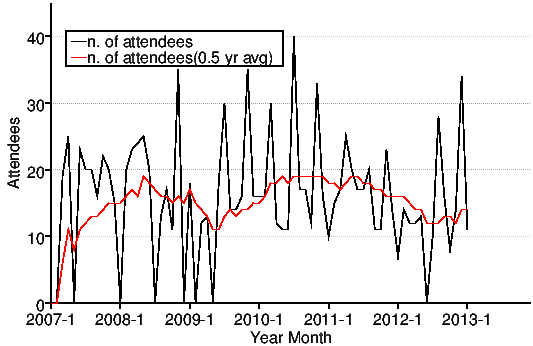
\includegraphics[width=.6\hsize]{image201212/memberanalysis/kansai.png}
    \end{center}
  \end{figure}
\end{frame}

\begin{frame}
  \frametitle{今年のイベント/お題}
  \begin{itemize}
  \item \color[rgb]{1,0,0}{月間Debian Policy}
    \begin{itemize}
    \item
      2章「Debianアーカイブ」, 3章「バイナリパッケージ」, \\
      4章「ソースパッケージ」, 5章「コントロールファイルとそのフィールド」,\\
      7章「パッケージ間の関連性の宣言」,12章「文章」
    \item 残りは
      1章, 6章, 8-11章, 付録A-E
    \end{itemize}
  \item \color[rgb]{0,0,1}{パッケージ関連}
    \begin{itemize}
    \item t-code, Konoha, ITP入門, News from EDOS, clang によるビルド
    \end{itemize}
  \item \color[rgb]{0,.5,.5}{イベント}
    \begin{itemize}
    \item 温泉合宿, 大統一Debian勉強会, OSC 2012 Kansai@Kyoto, KOF 2012
    \end{itemize}
  \end{itemize}
\end{frame}

\begin{frame}
  \frametitle{月刊Debian Policy について}
  \begin{description}
  \item[発端]\mbox{~}\\
    「月間物をやってみない?」という\sout{佐々木の無責任な}思いつきから
  \item[目的]\mbox{~}\\
    \begin{itemize}
    \item
      Debian の「深いところ」を学ぶ
    \item
      欲を言えば Debian JP Project の Web で公開されている翻訳を改善する
    \end{itemize}
  \item[現状]\mbox{~}\\
    \begin{itemize}
    \item 順調に(?)進んでおります.
    \item 折角みんなで読んだので, 翻訳の改善を push したいところですが...
    \end{itemize}
  \end{description}
\end{frame}

\begin{frame}
  \frametitle{翻訳関連}
  \begin{description}
  \item[発端] \mbox{~}\\
    \sout{OSS土下座組, 組長}岡野さん(@okano\_t)による精力的な活動もあり...
  \item[目的]
    \begin{itemize}
    \item 翻訳作業とその環境、査読プロセスなどの共有, 改善
    \item 翻訳結果の上流への貢献
    \end{itemize}
  \item[現状] \mbox{~}\\
    \begin{itemize}
    \item
      今年後半に盛り上がりました. \\
      今後も機会があれば継続していきたいですね.
    \item ...DSA更新はどうしましょうかね...
    \end{itemize}
  \end{description}
\end{frame}

\begin{frame}
  \frametitle{定例ネタ(パッケージ作成, バグ報告など)}
  \begin{exampleblock}{背景・目的}
    {\small{
        2007年度から関西でも Debian 勉強会を始動しています。
        \alert{短期的な目標は、Debian Developer(Debian開発者,以下DD) を増やすことです。}
        東京ではDebian勉強会が開催されてきましたが、一方の関西は、東京にくらべて DD の数が少ないです。 関西 Debian 勉強会は、DD と出会って GPG Key Sign をするチャンスを提供します。 また、勉強会を行うことを通して、Debian に関する知識を共有します。}}
    \vskip.5em
    \hspace*\fill{\small--- http://wiki.debian.org/KansaiDebianMeeting}
  \end{exampleblock}
  \begin{itemize}
  \item
    t-code のパッケージの改善, Konoha のパッケージ作成, ITP 入門
    \begin{itemize}
    \item \alert{モチベーション超重要}
    \end{itemize}
  \item NM プロセス中 -- 2名(佐々木, 倉敷さん)
  \item DD 以外での貢献
  \end{itemize}
\end{frame}

\takahashi[50]{大いなる\\反省点}
\takahashi[150]{運営}

\takahashi[25]{河田さんの獅子奮迅の活躍}
\takahashi[25]{運営フローの見直し@忘年会}

\begin{frame}
  \frametitle{イベント}
  \begin{itemize}
  \item 定例は以下の通り
    \begin{description}
    \item[OSC Kansai@Kyoto] \mbox{~}\\
      来年も 8 月?
    \item[KOF 2013] \mbox{~}\\
      来年も 11 月?
    \item[大統一Debian勉強会] \mbox{~}\\
      来年は関東で開催予定です. 参加費用用意しておこうね.
    \end{description}
  \item 課題:
    \begin{itemize}
    \item 申請担当者は?
    \item ブース展示/発表をどうするか?
    \end{itemize}
  \end{itemize}
\end{frame}

\section{ 2013年の企画 }
\takahashi[50]{ 2013年の企画 }

\begin{frame}
  \frametitle{2013年の企画}
\end{frame}

\takahashi[25]{ そんなこんなで }

\takahashi[25]{ 来年も頑張りましょう }

\takahashi[50]{  }


\end{document}
%%% Local Variables:
%%% mode: japanese-latex
%%% TeX-master: t
%%% outline-regexp: "\\([ 	]*\\\\\\(documentstyle\\|documentclass\\|emtext\\|section\\|begin{frame}\\)\\*?[ 	]*[[{]\\|[]+\\)" ***
%%% End:
